\section{Technischer Bericht}

\subsection{Einleitung und Übersicht}

\subsection{Was ist Xamarin?}


\subsection{Was ist die Methode 635?} \label{subsec:methode_635_desc}
Die gesamte Beschreibung der Methode 635 wurde von \href{https://kreativitätstechniken.info/6-3-5-methode/}{kreativitästechniken.info} \cite{methode-635} übernommen. 


Die Methode 635 (auch Methode 6-3-5 geschrieben) ist eine Brainwriting-Kre\-ati\-vi\-täts\-technik. Der Name leitet sich aus den drei wesentlichen Eigenschaften der Methode ab: jeweils 6 Teilnehmer erhalten ein Blatt Papier, auf dem sie je 3 Ideen notieren und die Blätter dann insgesamt 5 mal weiterreichen.

\subsubsection*{Anwendungsgebiete der Methode 635}
Die Methode 635 ist eine Variante des Brainwriting. Sie eignet sich besonders für die erste Phase im kreativen Prozess. Dabei werden zunächst Ideen gesammelt ohne dass eine Bewertung stattfindet. Im Idealfall können so in kurzer Zeit 108 Ideen entstehen. Die Aufforderung, bestehende Ideen aufzugreifen und weiterzuentwickeln macht die Methode 635 zu einer konstruktiven Kreativitätstechnik. Gleichzeitig kann die Kreativität durch die strukturierte Form aber auch gebremst werden. In der Praxis entstehen daher oft etwas weniger Ideen.

\subsubsection*{Vorgehen bei der Methode 635}
Zunächst erklärt der Moderator die Regeln der Methode 635, führt die Teilnehmer in das Ausgangsproblem ein und ist im Folgenden verantwortlich für die Zeitmessung. Sobald die Teilnehmer über die Ausgangsfrage oder -problem aufgeklärt sind, startet der Moderator die erste von sechs Runden. In jeder Runde werden die Teilnehmer aufgerufen, die oberste noch freie Zeile, bestehend aus 3 Kästchen, mit ihren Ideen zu füllen. Dabei sollten die Teilnehmer die Ideen der Vorgänger aufgreifen, erweitern und/oder weiterentwickeln ohne die Ideen zunächst zu bewerten. Nach einer festgelegten Zeit von beispielsweise 5 Minuten beendet der Moderator die Runde. Die Teilnehmer reichen ihr Arbeitsblatt im Uhrzeigersinn an ihren Sitznachbarn weiter und eine neue Runde beginnt. Im Idealfall sind nach 6 Runden genau 6*18 = 108 Ideen entstanden. In Realität ist die Anzahl aufgrund von doppelten oder leeren Einträgen wahrscheinlich etwas geringer. Dennoch sollten nun eine Vielzahl von Ideen vorliegen.


Nun kann eine Diskussion, Analyse und Bewertung der Ideen erfolgen.

\newpage

% Hier soll beschrieben werden wie der technische Bericht aufgebaut ist und was die Kapitel beinhalten.

\subsection{Vorstudie}
In der Vorstudie beschäftigten wir uns zuerst mit der Methode 635 an sich, um ein Gefühl dafür zu bekommen, wie es ist, diese selbst an einem konkreten Problem zu nutzen. 

Weiter beschäftigten wir uns mit Xamarin. Hierbei war vor allem der Entscheid zwischen Xamarin.Forms und Xamarin native von grosser Bedeutung, da dieser im späteren Projektverlauf kaum mehr rückgängig zu machen ist.

Ein weiterer Teil der Vorstudie bestand darin eine passende Umgebung  für das automatische Deployen der Xamarin Applikation zu finden. 

Zum Schluss der Vorstudie beschäftigten wir uns mit der Frage, welches Backend wir für unser Projekt verwenden sollten.

Einige wichtige Punkte und Entscheide waren stark von der Vorstudie abhängig.Es war daher entscheidend, bei der Vorstudie sorgfältig zu arbeiten.


\subsubsection{Erste Erfahrungen mit der Methode 635} \label{subsub:erste_erfahrungen_mit_methode_635}
Bevor wir uns mit den technischen Details der Umsetzung zur Cross-Plattform App auseinander gesetzt haben, spielte jeder der beiden Projektmitgliedern die Methode 635, wie in Kapitel \ref{subsec:methode_635_desc} beschrieben, mit seiner Familie, Bekannten oder Freunden einmal durch. 

Dabei wurden folgende persönliche Erfahrungen und Beobachtungen gemacht:

\begin{description}[leftmargin=!,labelwidth=\widthof{\bfseries Interessante Methode}]
	\item[Diskussion gestartet] Schon nach 2-3 Runden konnte beobachtet werden, dass sich spannende Diskussionen zum gestellten Problem entwickelten. Die Teilnehmer mussten sogar angehalten werden die Diskussionen auf dem Papier weiterzuführen, da sonst die Aussagen verloren gehen.
	\item[Interessante Methode] Die Teilnehmer empfanden die Methode 635 als spannend und interessant. Durch die einzelnen Teilnehmer waren auch verschiedenste Blickwinkel auf das Problem vertreten, was wiederum zu unterschiedlichsten neuen Ideen führe.
	\item[Wertung einführen] Was allerdings als kleiner Nachteil empfunden wurde, war der Umstand, dass die Methode 635 in der original Version keine Möglichkeit für Wertungen bietet. 
	
	Als Mensch bildet man sich während des Lesens der einzelnen Ideen automatisch eine Meinung darüber und wird dadurch stark dazu verleitet, eine wertende Bemerkung statt einer neuen oder angepassten Idee zu schreiben.
	
	Eine mögliche Verbesserung könnte darin bestehen, ein Möglichkeit für Wertungen der Ideen einzuführen. Dies könnte so aussehen, dass man neben dem Text auch ein Label (z.B. Pro oder Contra) und die Idee, welche man bewerten will, auswählen kann.
\end{description}

\subsubsection{Xamarin.Forms oder Xamarin native?}
%TODO würde hier die Vorteile und Nachteile von Forms und native zueinander erklären. Die Begründung warum wir uns für das eine entschieden haben, würde ich allerdings ins Architekturentscheide nehmen -> daher auch gleicher Titel im Dokument Architekturentscheide.

\subsubsection{Visual Studio App Center}


\subsubsection{Backend-Technologie}
Das Play Framework \cite{PlayFramework} ist ein, unter der Apache 2 Lizenz stehendes, Web Application Framework. Es folgt dem MVC-Pattern und erleichtert das Erstellen von Webanwendungen. Durch den Aufbau ermöglicht es dem Entwickler unter anderem auf einfache Art und Weise eine RESTful API zu schreiben. 

Play basiert auf einer zustandslosen und schlanken Architektur. Da es auf Akka aufgebaut ist, nützt es eine vollständig asynchrones I/O. Ausserdem bietet Play minimalen Ressourcenverbrauch. 

Sobald am Code eine Änderung vorgenommen wurde, wird der Server automatisch neugestartet, was die Produktivität des Entwicklers  weiter erhöht.

Jeglicher Code, welcher nicht kompiliert werden konnte, wird zudem im Browser angezeigt und man weiss als Entwickler sofort auf welcher Zeile man nachbessern muss. 

Seit der Version 2.0 des Play Frameworks ist der Framework Core in Scala geschrieben und als Build Tool wird SBT verwendet. Für das Testen stehen verschiedene Test Frameworks sowohl für Java als auch für Scala zur Verfügung. Mittels Scalatest oder JUnit können Unit Tests für beide Sprachen geschrieben werden. Es ist auch möglich Tools wie scoverage für die Code Coverage zu verwenden. 

\newpage

\subsection{Anforderungsspezifikation}

\subsubsection{Funktionale Anforderungen}

\paragraph{Brief Use-Cases}

Im Folgenden ist das Use-Case-Diagramm dargestellt.
\begin{figure}[h]
	\centering
	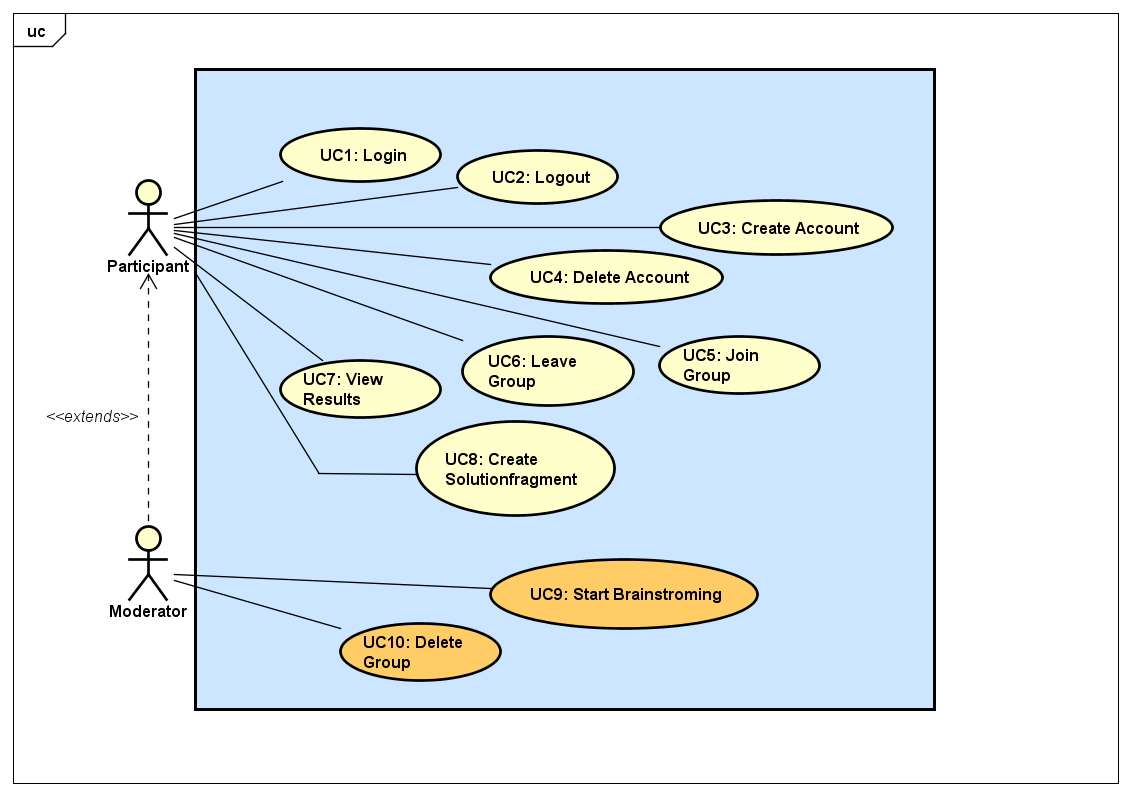
\includegraphics[width=1\linewidth]{img/anforderungen/UC-Methode635}
	\caption{Use-Case-Diagramm}
	\label{fig:ucmethode-635}
\end{figure}

Jeder Use-Case hat den nachfolgend kurz (\textit{briefly}) beschriebenen  Funktionsumfang. Die Hauptaktivitäten UC7-9 sind am Schluss \textit{fully-dressed} beschrieben.

\begin{basedescript}{%
		\desclabelstyle{\multilinelabel}
		\desclabelwidth{4.5cm}}
	\item[\textit{UC1: }Login] Als Participant möchte ich mich mit Benutzernamen und Passwort in das System einloggen können.
	\item[\textit{UC2: }Logout] Als eingeloggter Participant will ich mich ausloggen, sodass das Startfenster wieder erscheint.
	\item[\textit{UC3: }Create Account] Als Benutzer der Applikation möchte ich mich registrieren können.
	\item[\textit{UC4: }Delete Account] Als Benutzer will ich meinen erstellten Account wieder löschen können.
	\item[\textit{UC5: }Join Group] Als Participant will ich einer bereits existierenden Gruppe beitreten können.
	\item[\textit{UC6: }Leave Group] Als Participant will eine beigetretene Gruppe verlassen können.
	\item[\textit{UC7: }View Results] Als Participant will ich, nachdem eine Brainstorming Session durchgeführt wurde, das Resultat meiner Gruppe einsehen können.
	\item[\textit{UC8: }Create\\Solutionfragment] Als Participant will ich während einer Brainstorming Session ein Lösungsfragment erstellen und einreichen können. 
	\item[\textit{UC9: }Start \\Brainstorming] Als Moderator will ich eine Brainstorming Session starten.
	\item[\textit{UC10: }Create Group] Als Moderator will ich eine Gruppe erstellen können. 
	\item[\textit{UC11: }Delete Group] Als Moderator will ich eine Gruppe löschen können.
\end{basedescript}

\paragraph{Fully-Dressed Use-Cases}


\paragraph{Abuse-Cases}
%Abuse cases?
Um einem Missbrauch der Applikation entgegenzuwirken, sind neben den Use-Cases auch Abuse-Cases definiert. Diese helfen, mit unangebrachtem Inhalt und unangebrachter Verwendung umzugehen.
\begin{basedescript}{%
		\desclabelstyle{\multilinelabel}
		\desclabelwidth{4.5cm}}
	\item[\textit{AC1: }Unangebrachte Lösungsfragmente] Ein Participant könnte unangebrachte Inhalte in einer Gruppe hinzufügen. Um dies zu verhindern, könnte eine die Applikation um eine Funktion erweitert werden, die es dem Moderator erlaubt, Benutzer auszuschliessen.
\end{basedescript}

%Sequence diagram
\paragraph{Sequenzdiagramm}
Der Ablauf der Kernlogik ist der Abbildung \ref{fig:seq-methode635} zu entnehmen. Darin ist der Prozess vom Erstellen der Gruppe (UC10) bis zum Abschliessen der Brainstorming Session modelliert.
\begin{figure}[h]
	\centering
	\makebox[\textwidth][c]{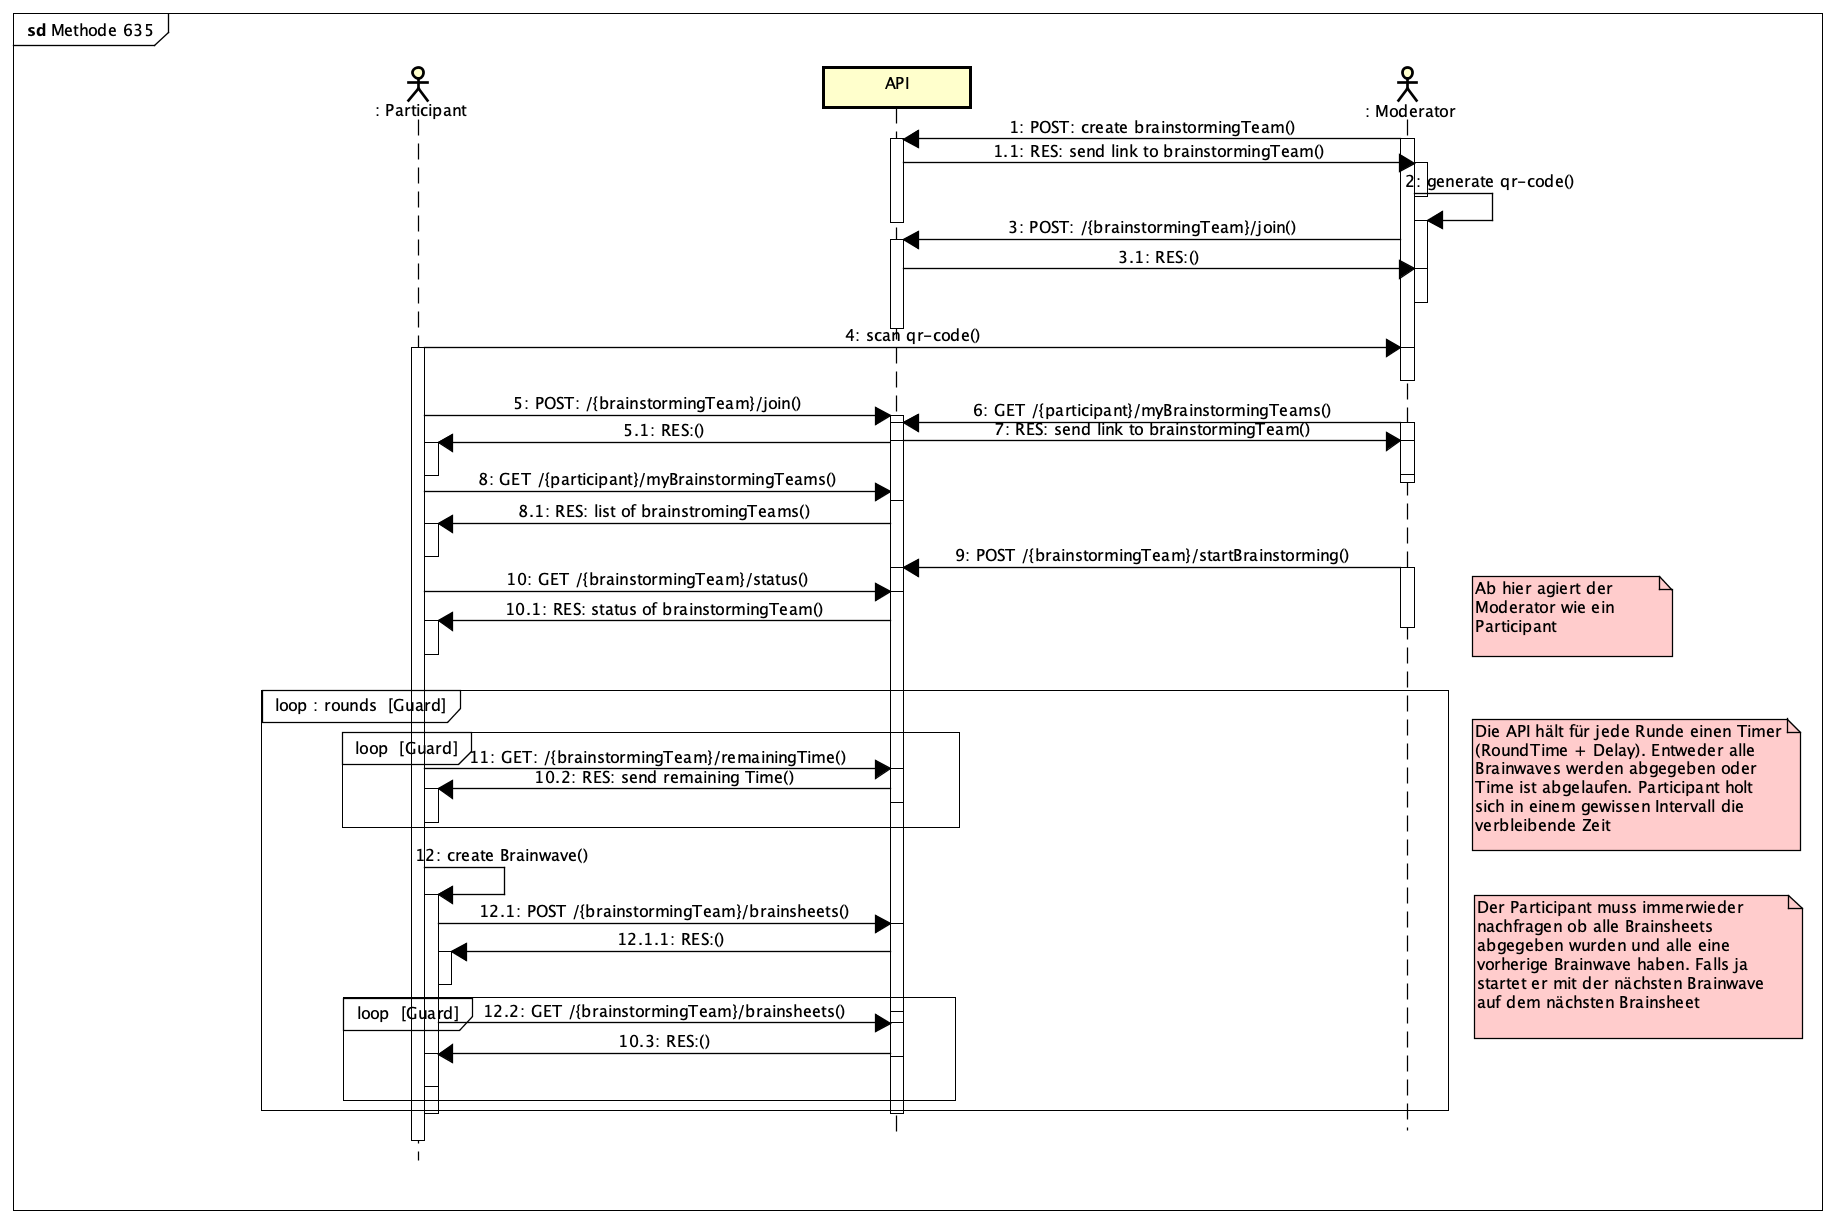
\includegraphics[width=1.2\linewidth]{img/anforderungen/Seq-Methode635}}
	\caption{Sequenzdiagramm}
	\label{fig:seq-methode635}
\end{figure}


\subsubsection{Nicht-Funktionale Anforderungen}
Beim Thema Nicht-Funktionale Anforderungen halten wir uns an die Standards ISO 9126\cite{ISO9126} bzw. dessen Nachfolger ISO 25010\cite{ISO9126_ISO25010}. Beide ISO-Normen sind sich sehr ähnlich und liefern eine gute Checkliste für jegliche Art von Systemanforderungen.

\begin{figure}[h]
	\centering
	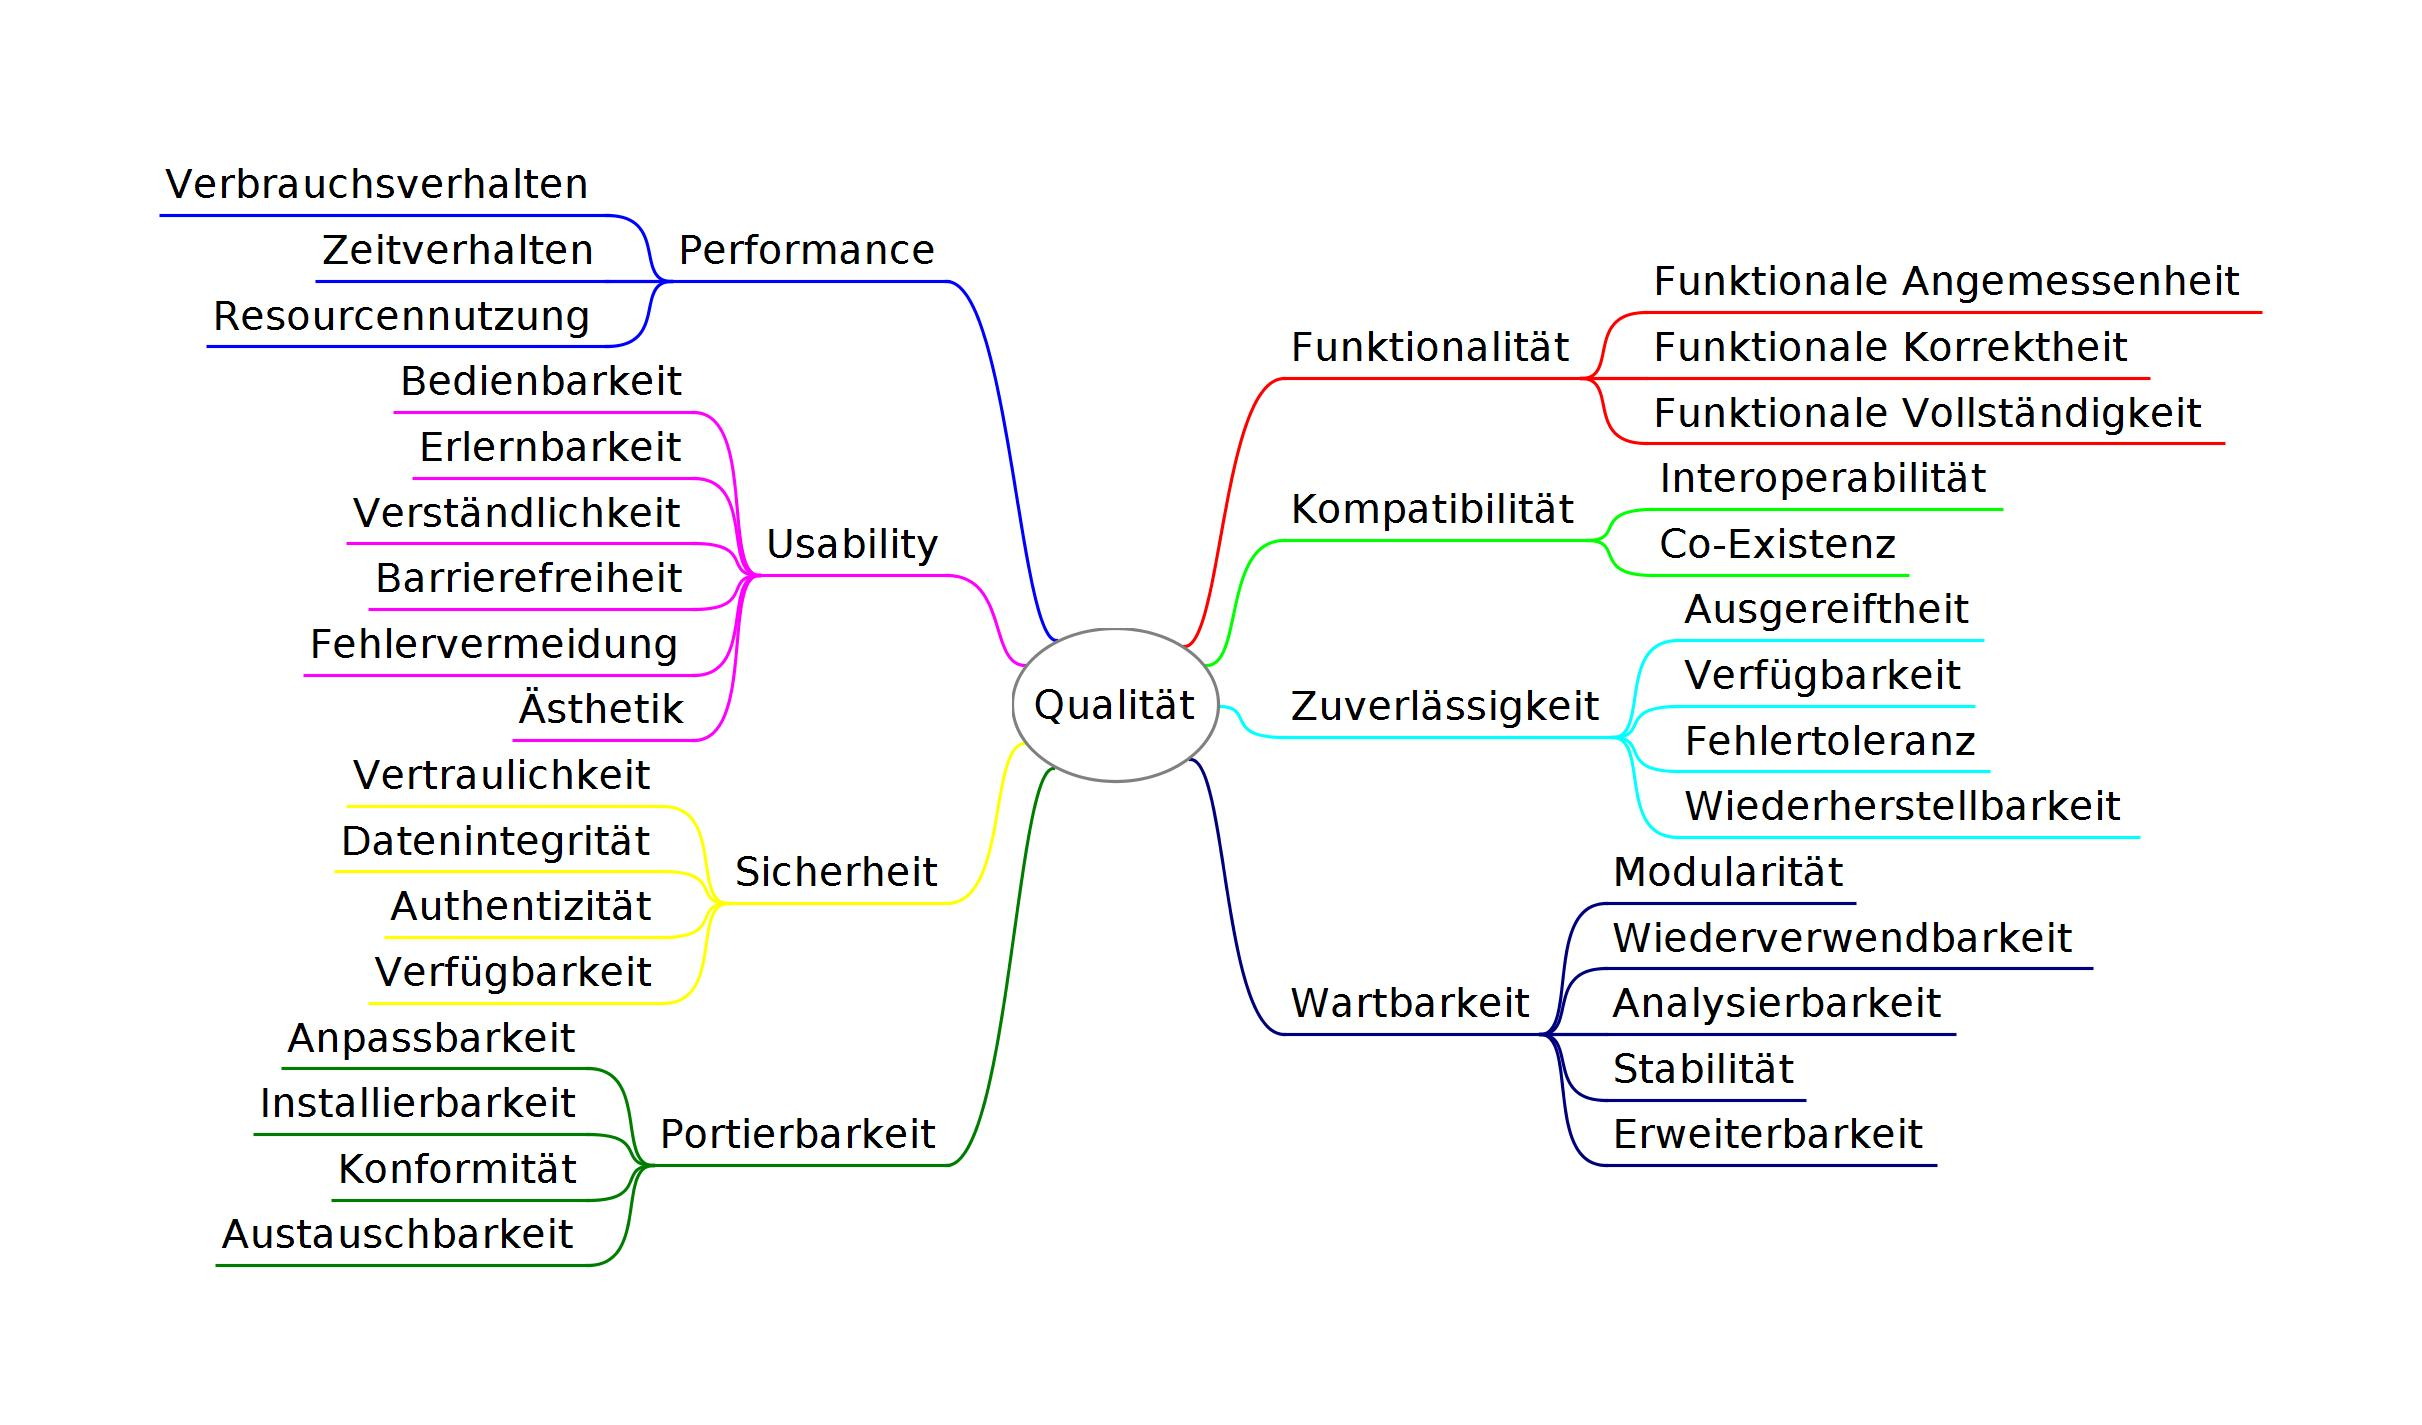
\includegraphics[width=1\linewidth]{img/anforderungen/quality}
	\caption[Anforderungskategorien nach ISO 25010]{Anforderungskategorien nach  ISO 25010}
	\label{fig:ISO 25010}
\end{figure}

%TODO Bild Link: https://blog.seibert-media.net/blog/2018/05/14/qualitaet-funktionale-und-nichtfunktionale-anforderungen-in-der-software-entwicklung/

Diese Normen sind sehr umfangreich gestaltet. Wir werden uns daher auf die, für uns, wichtigsten Anforderungen konzentrieren. Um genaue und erfüllbare nicht-funktionale Anforderungen zu definieren, müssen die SMART-Kriterien \cite{SMART} erfüllt sein. 

\begin{description}[leftmargin=!,labelwidth=\widthof{\bfseries Wiederverwendbarkeit}]
	\item[Ressourcennutzung] Die internen Ressourcen Kamera, Dateisystem dürfen nur bei effektivem Bedarf benützt werden. Die CPU-Ressourcen\-nutzung darf im Durchschnitt pro Minute maximal zu 40\% in Anspruch genommen werden.\footnote{Referenzsystem Android: Huawei P10 mit Android Version 8.0.0 mit Hisilicon Kirin 960 CPU und 4GB RAM}\footnote{Referenzsystem iOS: iPhone 6 mit iOS Version 12 mit Dual-core 1.4 GHz Typhoon CPU und 1GB RAM}
	
	\item[Bedienbarkeit] Wenn eine Aktion länger als 1-2s geht, soll dem User ein Wartesymbol angezeigt werden. 
	
	\item[Ästhetik] Die Benutzeroberflächen der Applikation sind so gestaltet, dass die Elemente wiedererkennbar sind (Buttons haben gleichen Stil, leere Textfelder haben Platzhalter). 
	
	\item[Vertraulichkeit] Die Daten einer Brainstorming Session können nur von der zugehörigen Gruppe eingesehen werden. 
	
	\item[Anpassbarkeit] Die Anpassung bestehender oder Integration neuer Brain\-storming-Methoden muss gewährleistet sein.
	
	\item[Installierbarkeit] Die Installation der Applikation auf einem Endgerät erfolgt durch das Ausführen eines *.apk oder *.app. Dieser Prozess soll unter 1 Minute geschehen.
	
	\item[Co-Existenz] Sollte zu einem späteren Zeitpunkt entschieden werden ein Web-Frontend zu programmieren, muss dieses co-existent mit der Xamarin Applikation existieren können.
	
	\item[Wiederherstellbarkeit] Im Falle eines fehlerhaften Features, muss es innerhalb eines Werktages möglich sein, die Applikation wieder auf den letzten funktionierenden Stand zurück zu holen und erneut zu deployen.	
	
	\item[Wiederverwendbarkeit] Die Auswertung von 'Duplicated Code' in SonarQube soll unter 8\% liegen. Dies deutet auf eine hohe Wiederverwendbarkeit hin, denn ansonsten müsste der Code kopiert werden. 
	
	%TODO: Referenz auf Use Cases
	\item[Analysierbarkeit] Das Ausführen eines Use-Cases muss durch Analyse von Logfiles erkennbar sein.
\end{description}

\newpage

\subsection{Domainanalyse}

Das Domain-Modell besteht grob aus zwei Teilen: den Benutzern und der Brainstorming Methodik. 

Dabei bilden mehrere Participants ein \textit{Brainstorming Team}. Diese wird von einem der Participants, dem \textit{Moderator}, gegründet.  Das Team hat die Möglichkeit, ein oder mehrere \textit{Brainstorming Findings} zu erarbeiten. Dies entspricht einer gesamten Durchgang der Methode. Der Moderator erstellt diese und hat die Möglichkeit, die Anzahl von Ideen sowie die erste Rundenzeit zu konfigurieren. Jede weitere Runde wird um eine Minute verlängert.

Das \textit{Brainsheet} entspricht einem physikalischem Blatt, das herumgegeben wird. In der Standardkonfiguration 635 existieren also 6 Sheets (weil 6 Teilnehmer dabei sind).

Eine \textit{Brainwave} ist das Produkt jedes Participants am Ende einer Runde. Es gehört in ein Brainsheet, das jede Runde an den nächsten Participant weitergegeben wird. In der Standardkonfiguration besteht eine Brainwave aus 3 Ideen (6\textbf{3}5).

Die \textit{Idea} ist ein effektiv erarbeiteter Teil einer Brainwave. Im Normalfall ist eine Idee simpler Text (\textit{NoteIdea}), wobei weitere Typen von Ideen (Bild, Weblink und Zeichnung) durch das verwendete Design erdenklich sind. 
\begin{figure}[h]
	\centering
	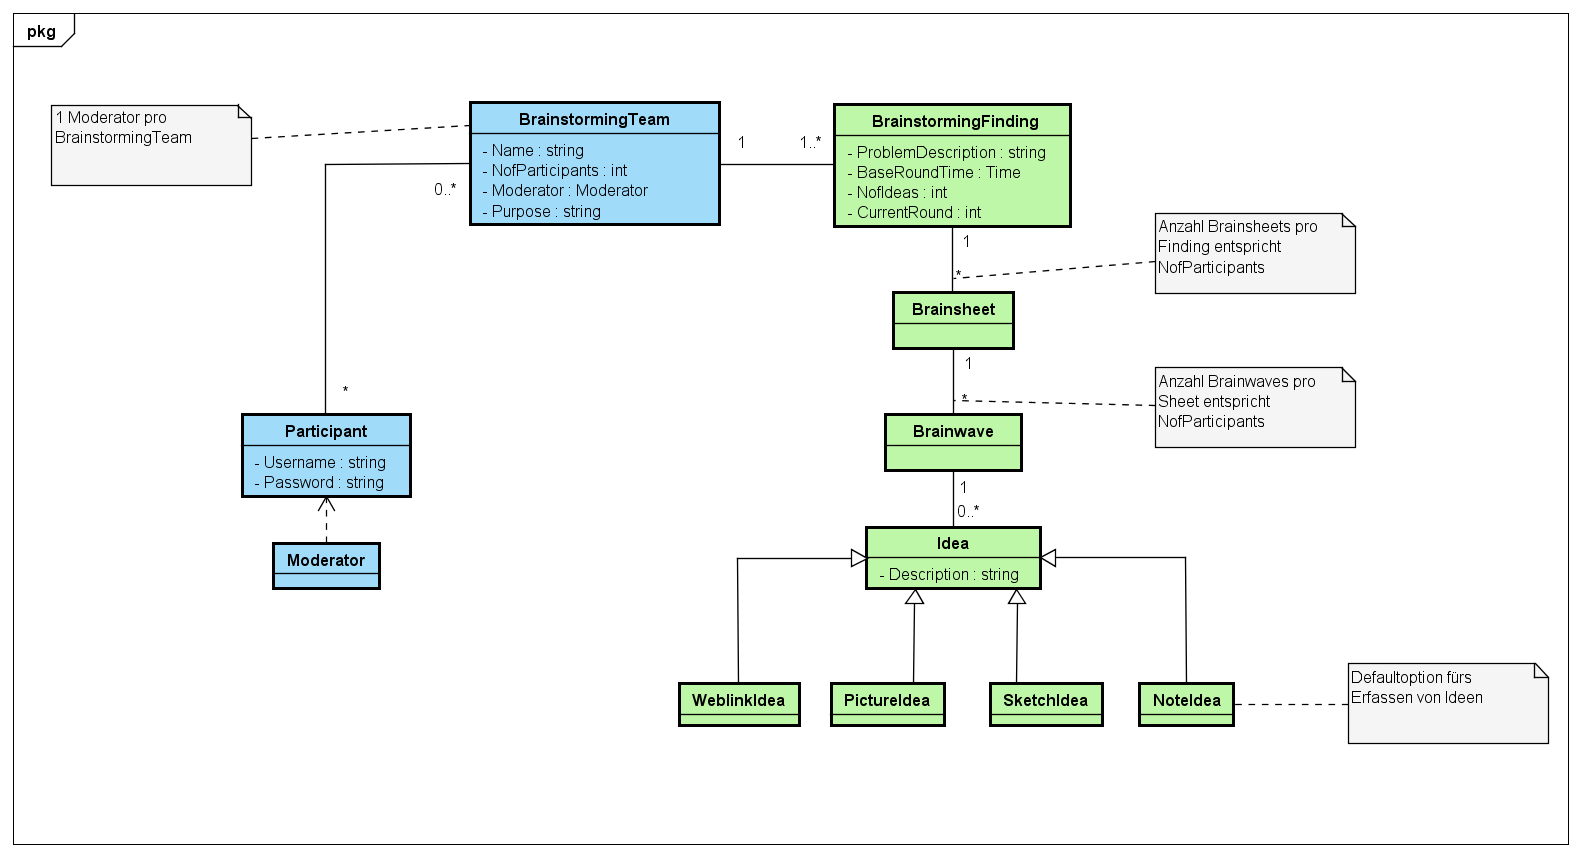
\includegraphics[width=1\linewidth]{img/domain-analyse/DomainModell-Methode635}
	\caption{Domain Modell BrainingOutOfBox}
	\label{fig:domainmodell-methode635}
\end{figure}

\newpage

\subsection{Architekturdokumentation}
\label{architektur}
In diesem Kapitel gehen wir detailliert in die Architektur und das Deployment unseres Projektes ein.

\subsubsection{Logische Architektur}
Wir teilen die Architektur des gesamten Systems in drei Schichten auf. In der Abbildung \ref{fig:architektur-methode635} sind diese als Presentation-, Businesslogic- und Persistence-Schicht zu erkennen.

\begin{figure}[h]
	\centering
	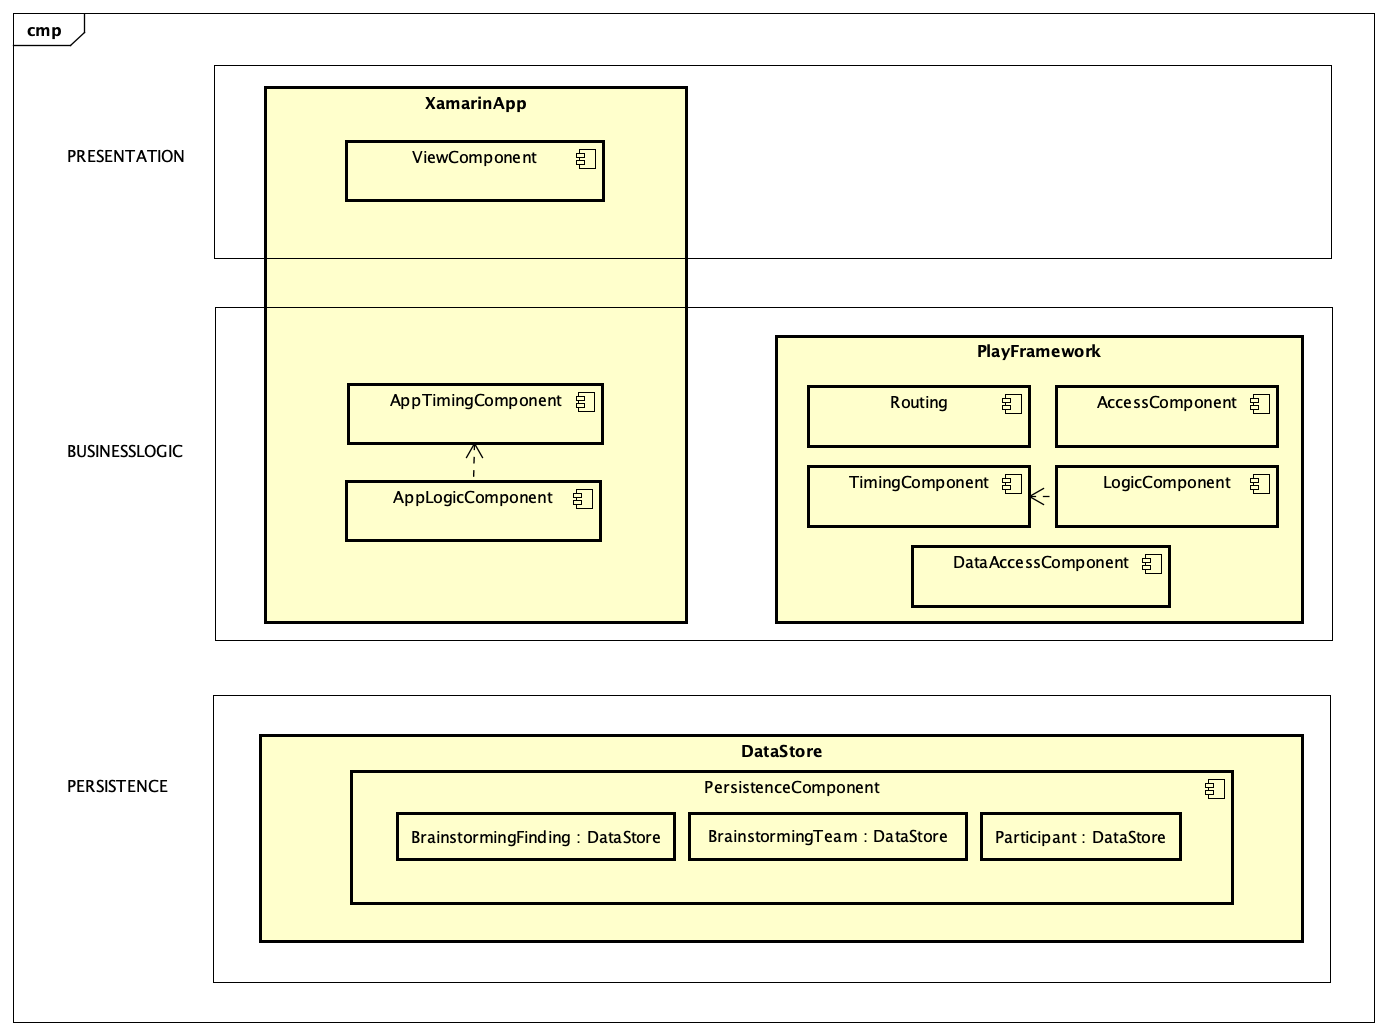
\includegraphics[width=1\linewidth]{img/architektur/CD_Methode635}
	\caption{Logische Architektur BrainingOutOfBox}
	\label{fig:architektur-methode635}
\end{figure}

Die Präsentationsschicht ist die Schicht über die der Benutzer mit der Xamarin App kommuniziert. Konkreter gesagt, umfasst diese die verschiedenen View-Komponenten, welche für das Aussehen der App verantwortlich sind. Jegliche Interaktionen über die Oberfläche werden anschliessend in der Schicht der Businesslogic weiter verarbeitet. In dieser Schicht haben wir zum einen wieder unsere Xamarin App, welche selbst Logik-Komponenten wie die Timing-Komponente oder weitere App spezifische Logik-Komponenten enthält.

Die AppLogic-Komponente ist für das korrekte Verarbeiten und Weiterleiten der Eingaben an das PlayFramework verantwortlich.

Die AppTiming-Komponente ist zuständig für das Zeitmanagement während den einzelnen Runden. Diese Komponente überwacht daher die noch verbleibende Zeit.

Auf der anderen Seite haben wir das PlayFramework, welches wiederum Access-Komponenten, Routing-Komponenten, eine Timing-Komponente, Logik-Komponenten und eine DataAccess-Komponente enthält.

Die Timing-Komponente und die Logic-Komponente haben die selben Aufgaben wie ihre Gegenstücke in der Xamarin App. Auch hier verwalten diese das Zeitmanagement während den einzelnen Runden und stellen sicher, dass nach Ablauf der Zeit oder sobald alle \textit{BrainSheets} abgegeben wurden, eine neue Runde beginnt. Des Weitern ist die Logic-Komponente zum Beispiel verantwortlich, dass ein \textit{Participant} einer Gruppe nicht zweimal beitreten kann oder diese verlassen kann, wenn er sie schon einmal verlassen hat. 

Die DataAccess-Komponente stellt sicher, dass jegliche Daten korrekt geladen oder gespeichert werden.

Mit der Schicht der Datenhaltung (Persistence) haben wir eine Schicht zur Verfügung, welche eine Persistence-Komponente hält. 

Konkret steht uns je ein DataStore für die \textit{BrainstormingFindings}, für die \textit{BrainstormingTeams} und für die \textit{Participants} zur Verfügung.


\paragraph*{Komponenten}
Nachfolgend sind nochmals alle Komponenten aufgelistet und kurz beschrieben. Für eine ausführlichere Beschreibung ist der Text oberhalb zu lesen.

\begin{description}[leftmargin=!,labelwidth=\widthof{\bfseries DataAccessComponent}]
	\item[ViewComponent] Die View-Komponenten der Xamarin App sind für das korrekte Anzeigen der Informationen verantwortlich. Sie definieren das Aussehen der Applikation.
	\item[AppTimingComponent] Die Xamarin App hält in der logischen Schicht eine Timing-Komponente, welche dafür sorgt, dass ein \textit{BrainstormingFinding} nach Ablauf der Zeit abgesendet wird.
	\item[AppLogicComponent] Die Logik-Komponente der Xamarin App regelt weitere Logik, wie z.B. den Zugriff auf das PlayFramework.
	\item[AccessComponent] Die Access-Komponente auf dem PlayFramework regelt den Zugriff mittels JWT-Token\cite{jwt}. JWT-Tokens werden bei erfolgreichem Login an den Benutzer der App gesendet. So kann sichergestellt werden, dass nur registrierte Benutzer mit dem PlayFramework interagieren können.
	\item[Routing] Die Routing-Komponente sorgt anhand der URL für das Aufrufen der korrekten Funktion.
	\item[TimingComponent] Wie die Xamarin App hält auch das PlayFramework eine Timing-Komponente, um den Zustand der Zeit verwalten zu können.
	\item[LogicComponent] In der Logik-Komponente werden die eigentlichen Funktionen geschrieben. Hier ist auch die Logik für den Austausch der Blätter untergebracht.
	\item[DataAccessComponent] Die DataAccess-Komponente stellt das Bindeglied zwischen dem PlayFramework und dem DataStore dar. Es ermöglicht erst den Zugriff auf die gespeicherten Daten.
	\item[PersistenceComponent] Die Persistence-Komponente regelt das korrekte und dauerhafte Speichern in die einzelnen DataStores.
\end{description}


\subsubsection{Deployment}
Wie in der Abbildung \ref{fig:deployment-methode635} zu sehen ist, besteht unser System aus zwei physikalischen Geräten. Das ist zum einen der Client und zum anderen der BackendNode. Diese beinhalten jeweils sogenannte \textit{DeploymentUnits} (DU). 

\begin{figure}[h]
	\centering
	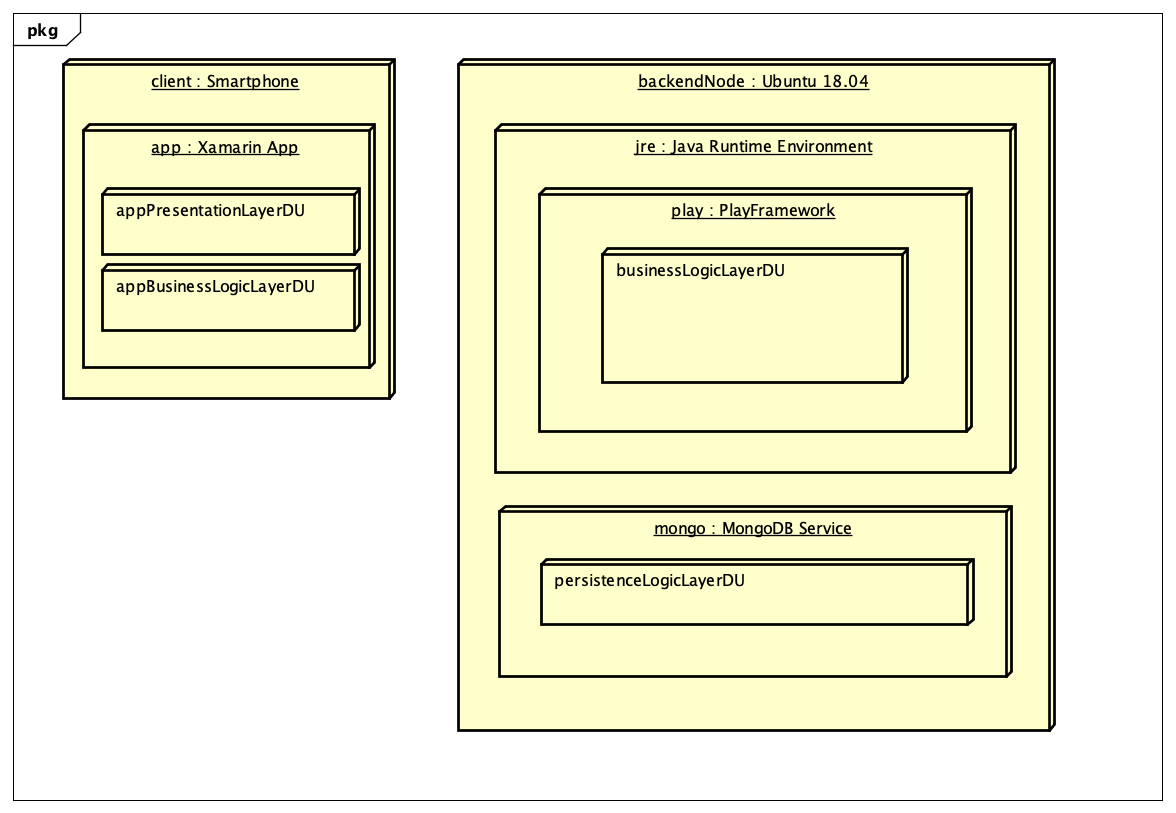
\includegraphics[width=1\linewidth]{img/deployment/DD_Methode635}
	\caption{Deploymentdiagramm BrainingOutOfBox}
	\label{fig:deployment-methode635}
\end{figure}

Beim Client handelt es sich um das Smartphone des jeweiligen Benutzers. Auf seinem Smartphone läuft die Xamarin App, welche wiederum die appPresentationLayerDU und die appBusinessLogicLayerDU hält.

Der BackendNode ist ein Ubuntu 18.04 auf dem ein Java Runtime Environment (JRE) installiert ist. Innerhalb der JRE läuft das PlayFramework, in dem wiederum die businessLogicLayerDU läuft.

Zudem ist auf dem BackendNode ein MongoDB Service installiert, welche  die persistenceLogicLayerDU beinhaltet.

\paragraph*{Komponenten}
Nachfolgend sind nochmals alle DeploymentUnits aufgelistet und kurz beschrieben.
\begin{description}[leftmargin=!,labelwidth=\widthof{\bfseries appBusinessLogicLayerDU}]
	\item[businessLogicLayerDU] Die businessLogicLayerDU enthält alle Komponenten, welche in Abbildung \ref{fig:architektur-methode635} in der Businesslogic-Schicht im PlayFramework eingezeichnet sind.
	\item[persistenceLogicLayerDU] Die persistenceLogicLayerDU beinhaltet alle Komponenten der Persistence-Schicht, welche in Abbildung \ref{fig:architektur-methode635} zu sehen ist.
	\item[appPresentationLayerDU] Die appPresentationLayerDU enthält alle Komponenten, welche in Abbildung \ref{fig:architektur-methode635} in der Präsentationsschicht liegen.
	\item[appBusinessLogicLayerDU] Die appBusinessLogicLayerDU enthält alle Komponenten, welche in Abbildung \ref{fig:architektur-methode635} in der Businesslogic-Schicht in der Xamarin App gezeichnet sind.
\end{description}

\newpage

\subsection{Architekturentscheide}
Jegliche Entscheide, welche wir während dem Projekt getroffen haben, sind hier detailliert begründet. Auch Gedanken oder Ideen, welche wir während der Analysephase hatten, dann aber verworfen haben, sind hier aufgeschrieben.

\subsubsection{Erste Erfahrungen mit der Methode 635}
Wie in Kapitel \ref{subsub:erste_erfahrungen_mit_methode_635} beschrieben, tendiert der Mensch dazu, die Ideen der anderen Teilnehmer automatisch zu bewerten. Als mögliche Lösung wurde die Integration einer Bewertungsmöglichkeit beschrieben.


Wir haben uns allerdings darauf geeinigt, dass wir die originale Version, also ohne die Möglichkeit für eine Wertung, als Vorlage nehmen und diese auch so in unserer Cross-Plattform Applikation umsetzen. 


Die Integration einer Bewertungsmöglichkeit wird als optionales Feature angesehen und lediglich bei genügend Restzeit im Projekt umgesetzt.

\subsubsection{Xamarin.Forms oder Xamarin native}
Für diesen Entscheid galt es zu evaluieren, welche User Controls für unsere Applikation die exotischsten sind. Dies, weil Xamarin.Forms eine Menge an Standard-Controls anbietet, die vom Framework selber in das jeweilige Betriebssystem konvertiert werden. Sind alle vorgesehenen Benutzerelemente in Forms enthalten, sparen wir uns die Zeit, betriebssystemspezifische Elemente zu entwickeln. 

Für unser Projekt haben wir folgende Benutzerelemente als exotisch oder kritisch definiert:
\begin{itemize}
	\item Canvas Control für Zeichnen einer Idee
	\item Camera Funktion für das Erkennen von Quick Response-Codes (QR-Codes)
	\item Verarbeitung und Generierung von QR-Codes
\end{itemize}

Nach einer Recherche stellte sich heraus, dass sich ein Canvas View von Google namens SkiaSharp \cite{skiaSharp} eignet. Darauf lässt sich gemäss der Dokumentation zeichnen sowie definierte Formen einfügen. Dies könnte auch für eine Erweiterung spannend sein, in der Patterns in UML als Vorlage angeboten werden können.

Für die Kamera-Funktionalität steht ein NuGet-Packet (Xam.Media.Plugin \cite{xam-media-plugin}) bereit, das uns diese Arbeit abnehmen wird.

Das Generieren und Lesen der QR-Codes ist an sich kein Problem von Xamarin.Forms, denn grundsätzlich müssen die von der Kamera generierten Files eingelesen und ins entsprechende QR-Code-Tool eingefügt werden. Hierfür eignet sich das NuGet ZXing.Net (\cite{zxing.net}). 

Es stellte sich relativ rasch heraus, dass die gewünschten Funktionalitäten in Xamarin.Forms in ausreichender Qualität enthalten sind und uns das individuelle Entwickeln dadurch abgenommen wird.

\subsubsection{Backend-Technologie}
Neben den Vorteilen, wie der schlanken und zustandslosen Architektur des PlayFrameworks, dem asynchronen und nicht-blockierenden Verhalten und den vielen unterstützten Bibliotheken, haben wir uns hauptsächlich dafür entschieden, weil wir in anderen Projekten schon sehr gute Erfahrungen mit dem PlayFramework gemacht haben.

Ein weiterer Grund bestand darin, dass das PlayFramework nicht nur in Scala sondern auch in Java geschrieben ist. Mit Java kennen wir uns beide gut aus und mussten uns so keine neue Programmiersprache aneignen.

Da wir uns schon relativ früh für eine MongoDB als Datenbanksystem entschieden hatten, viel die Wahl für das Play Framework erst recht, als wir einen asynchronen MongoDB-Treiber für Java gefunden hatten.

\subsubsection{MongoDB als Datenbanksystem}
MongoDB (abgeleitet von humongous) ist eine dokumentorientierte \cite{MonogDBWikipedia}, einfache, dynamische und skalierbare NoSQL Datenbank \cite{MonogDBDZone}, welche von der MongoDB Inc. entwickelt wird \cite{MonogDB}. 

Die Basis für das Speichern von Informationen bilden die sogenannten Documents. Die Datenobjekte werden in separaten Documents innerhalb einer Collection (anders als bei traditionellen Relationalen Datenbanken in Spalten und Zeilen) gespeichert \cite{MonogDBDZone}. Mit den Documents können zudem  hierarchische Strukturen und Relationen sehr einfach gespeichert werden.

Der Vorteil einer MongoDB Datenbank liegt darin, dass zusammengehörige Informationen gemeinsam in einem Document gespeichert werden. Dies ermöglicht einen schnellen Zugriff auf die Daten mittels der MongoDB Query Language. Da MongoDB zudem ohne Schemas auskommt, ist es nicht nötig, die Datenbank offline zu nehmen, wenn man ein neues Feld einfügen möchte \cite{MonogDB}.

Weitere Vorteile sind laut \href{DZone.com}{DZone.com} die hohe Performance, Verfügbarkeit (durch Replikas) und Skalierung (durch Sharding). Da alle Informationen zusammen in einem Document gespeichert sind, sind auch keine Joins zu anderen Tabellen notwendig. Auch unterstützt MongoDB Funktionen für die Speicherung von Geoinformationen \cite{MonogDBDZone}.

Der Hauptgrund warum wir uns für MongoDB als Datenbanksystem entschieden haben, war die Tatsache, dass alle zusammengehörigen Informationen in einem Document abgelegt werden können. Auch die Möglichkeit hierarchische Strukturen (bei uns die \textit{Brainsheets}, \textit{Brainwaves} und \textit{Ideas}) einfach zu Speichern, hat uns viel Zeit erspart.

Die Mächtigkeit von relationalen Datenbanken im Bereich einer Auswertung, ist in unserem Projekt nicht notwendig. Daher haben wir auch von Beginn an auf das Paradigma der dokumentorientieren Datenbanken gesetzt. Grund warum wir uns schlussendlich für MongoDB und nicht für eine andere dokumentorientierte Datenbank entschieden haben ist, dass MongoDB Thema während dem Studium ist und wir schon einige Erfahrung damit hatten.

\subsubsection{Methode 635 als Peer-to-Peer-System}
Wir haben uns auch überlegt, die Cross-Plattform Applikation d.h. vor allem die Kommunikation zwischen den einzelnen Teilnehmer, als Peer-to-Peer System \cite{Peer2Peer} zu konzipieren.


Prof. Thomas Bocek, Professor für verteilte Systeme an der Hochschule Rapperswil, hat uns allerdings davon abgeraten. Ein verteiltes System sei immer komplexer und komplizierter als ein Server/Client System. Für diese geringe Anzahl von Teilnehmern, welche prinzipiell nur Messages austauschen, lohnt es sich nicht ein verteiltes System zu bauen. 


Daher haben wir uns für eine klassische Server/Client Architektur entschieden. Andere Varianten der Kommunikation, wie Webhooks oder Websockets werden daher nicht weiter verfolgt.

\subsubsection{Kommunikation zwischen Server und App}
Die Kommunikation zwischen dem zentralen Server und den Clients, also den Cross-Plattform Applikationen in unserem Fall, ist von grosser Bedeutung. Wegen der Problematik der Network Address Translation kurz NAT \cite{NAT} kann diese prinzipiell auf zwei Arten erfolgen: Entweder man verwendet Websockets \cite{WebSockets}, welche eine permanente Verbindung zwischen Server und Client öffnen oder die Kommunikation beginnt ausschliesslich beim Client. 


Wir haben uns für das stetige Abfragen von Informationen (Polling) entschieden, da es eine einfache Variante darstellt. Zwar werden dadurch vermeidbare Requests an den Server gesendet, da aber die Anzahl an Teilnehmer bzw. die Ressourcennutzung des Backends in einem vertretbaren Rahmen liegt, ist diese Polling-Variante völlig in Ordnung.  

\textbf{Zwei Beispiele für Polling in der Applikation}: Wenn ein Teilnehmer seine Ideen aufschreibt, fragt die Applikation den Server im Hintergrund in regelmässigen Abständen nach der verbleibenden Zeit für diese Runde ab.


Auch nach der Abgabe der aufgeschriebenen Ideen an den Server, muss der Teilnehmer warten, bis er die Ideen bzw. das Blatt seines Nachbarn bekommt. Dafür muss die Applikation immer wieder den Server fragen, ob der Nachbar überhaupt sein Blatt bzw. seine Ideen abgegeben hat. Bevor dies nicht geschehen ist, kann der Teilnehmer auch nicht weitermachen.


\textbf{Begründung in Zahlen:}
Bei diesen beiden Szenarien sendet die Applikation pro Sekunde einen Request an den Server. Wenn wir bei der Standardmethode von 6 Teilnehmern bleiben, wären das 6 Request pro Sekunde. Wenn wir nun noch annehmen, dass 50 gleichzeitige Ausführungen stattfinden, ergibt das 300 Requests pro Sekunde für eines der beiden Szenarien.


Laut den Release-Informationen zur Version 2.5 von Play \cite{Play25} ist das PlayFramework in der Lage 60'000 Requests pro Sekunde zu verarbeiten.


Nehmen wir nun diese 60'000 Requests als Basis für unsere Berechnung, entsprechen unsere 300 Requests gerade einmal 0.5\% der möglichen 60'000 Requests. Für beide Szenarien entsprechend das Doppelte, also 1\%.

\[\frac{300Requests}{1s}=\frac{1Request}{1s}\cdot6Participants \cdot50Brainstormings\]
\[0.5\%= \frac{\frac{300Requests}{1s} \cdot 100}{\frac{60000Requests}{1s}} = \frac{300 \cdot 100}{60000}\]

\textbf{Fazit:} Diese kleine Rechnung verdeutlich schon ziemlich stark, dass die Variante mit dem Polling das PlayFramework in keinster Weise an dessen Limit bringt. Selbst wenn die Anzahl an Teilnehmern oder gleichzeitigen Ausführungen erhöht wird, ist das PlayFramework im Stande die eingehenden Requests noch zu verarbeiten. Auch andere gleichzeitige Aufrufe an das PlayFramework können dann noch ausgeführt werden.

Sollte es dennoch jemals zu einer zu starken Ressourcennutzung durch das Polling kommen, könnte der Algorithmus so angepasst werden, dass dieser nicht jede Sekunde das Backend z.B. nach der verbleibenden Zeit abfragt sondern bei viel verbleibender Zeit nur alle 30 Sekunden und bei wenig verbleibender Zeit jede Sekunde.

Auf diese Weise kann die Anzahl an Requests drastisch reduziert werden.

\newpage


\subsection{Ergebnisse}

\subsection{Schlussfolgerungen}
\subsubsection{Ergebnisbewertung}
\subsubsection{Ausblick}